\documentclass[aspectratio=43]{beamer}
\usepackage[utf8]{inputenc}

%%%%%%%%%%%%%%%%%%%%%%%% THEME
\usetheme{material}
\useLightTheme
\usePrimaryBrown
\useAccentAmber

\usepackage{macros} % must come after theme

\title{\q Gates}
\keywords{\qcts}


\begin{document}

\begin{frame}
	\titlepage
\end{frame}


\begin{frame}{Table of contents}
	\begin{card}
		\tableofcontents
	\end{card}
\end{frame}


\section{Introduction}
\begin{frame}{Introduction}
    \begin{card}
    This week is focused on recalling some linear algebra notions that are very useful for designing quantum circuits. We will briefly recall the concept of Hermitian and Unitary operators.\\ Afterwards, we will go through some important one-qubit gates and their \qk representation, moving on to 2-qubit gates.\\Lastly, we will have exercises to practice these topics and make them feel more natural, as they are the backbone of what's to come!
    \end{card}
\pagenumber
\end{frame}

\section{Conjugate Transpose}
\begin{frame}{Conjugate Transpose $A^\dag$}
\begin{card}
    The Conjugate Transpose of a complex matrix $A$ (denoted $A^\dag$) is the transpose of $A$ ($A^T$) after we take the complex conjugate of each element of $A$. 
    Here's an example:
    \begin{equation*}
        \begin{bmatrix}1 + i & -1\\ 1 & -1 - i\end{bmatrix}^\dag
        =
        \begin{bmatrix}1 - i & 1\\ -1 & -1 + i\end{bmatrix}
    \end{equation*}
\end{card}
\begin{cardTiny}
    Recall that the complex conjugate of $a+bi$ is simply $a-bi$ (geometrically, it is the reflection of the complex number over the real axis in the complex plane).
\end{cardTiny}
\pagenumber
\end{frame}


\section{Hermitian Matrix}
\begin{frame}{Hermitian Matrix $A = A^\dag$}
\begin{card}
    Hermitian refers to complex matrices ($H \in \mathbb{C}^2$) that equal their complex conjugate: $A = A^\dag$.\\
    These are matrices whose eigenvalues are always real numbers ($\lambda \in \mathbb{R}$).
\end{card}
\begin{card}
    Try to verify the following example:
    \begin{equation*}
        A = \begin{bmatrix}1 & 2+i & 3\\2-i & 5 & i\\3 & -i & 1\end{bmatrix}
    \end{equation*}
    \begin{equation*}
    A^\dag = A \Rightarrow\text{ A is Hermitian}
    \end{equation*}
\end{card}
\pagenumber
\end{frame}

\section{Unitary Operators}
\begin{frame}{Unitary Operators}
    \begin{card}
        A Linear Transformation ($T$) allows the conversion from a vector space ($V$) to another ($W$) $T : W \rightarrow V$ such that:
        \begin{itemize}
            \item $T(v1+v2)=T(v1)+T(v2)$ : $v1, v2 \in V$
            \item $T(\gamma \times v)=\gamma \times T(v)$ for any scalar $\gamma$
        \end{itemize}
    \end{card}
    
    \begin{cardTiny}
        A Unitary Operator is a Linear Operator (an operator that performs a linear transformation), with the additional constraint that it is unitary: $AA^\dag=A^\dag A = I$.\\
        These means we can apply a unitary operator to a vector space twice and get the original vector space. We care about them because this is exactly how quantum gates operate!
    \end{cardTiny}
\pagenumber
\end{frame}


\section{\q Gates}
\begin{frame}{\q Gates}
\begin{card}
    A quantum gate is an analogy of classic gates and is also a useful paradigm to think about qubit manipulation.\\ Also known as quantum logic gates, they have the following properties:
    \begin{itemize}
        \item Reversible (applied twice result in the original state) unlike some classical gates (for example the OR gate)
        \item Represented by Unitary matrices
        \item Each gate is only applied to the same number of qubits (one-qubit gates, two-qubit gates, ...)
    \end{itemize}
    We will see some of the more common gates and how to use them in \qk, but more will come into play as your quantum knowledge increases.
\end{card}
\pagenumber
\end{frame}



\subsection{Hadamard}
\begin{frame}{Hadamard}
\begin{cardTiny}
    The Hadamard gate is applied to a single qubit. If your qubit is in a state $\ket{0}$, after the Hadamard, it will be in a superposition of $\osqrt\ket{0}+\osqrt\ket{1}$. If it is in $\ket{1}$ it will end up in $\osqrt\ket{0}-\osqrt\ket{1}$. It is essential to create a \textbf{superposition} from $\ket{0}$. Try to verify this using the vector version of the qubit and the following unitary operator:
    \begin{equation*}
        H=\osqrt\begin{bmatrix}1 & 1\\1 & -1\end{bmatrix}
    \end{equation*}
    Also, try to check that $HH^\dag=H^\dag H = I$.
\end{cardTiny}
\pagenumber
\end{frame}

\begin{frame}[fragile]{Hadamard in \qk}
\begin{card}
    After you have created your QuantumCircuit \mintinline{python}{circuit}
    \begin{minted}{python}
# Create a Quantum Register with 2 qubits
qr = QuantumRegister(2) # 1 would suffice

# Create a Quantum Circuit from the qr and cr registers
circuit = QuantumCircuit(qr, cr)

# H gate on qubit 0
circuit.h(qr[0])
    \end{minted}
    \begin{center}
        

\tikzset{every picture/.style={line width=0.75pt}} %set default line width to 0.75pt        

\begin{tikzpicture}[x=0.75pt,y=0.75pt,yscale=-1,xscale=1]
%uncomment if require: \path (0,300); %set diagram left start at 0, and has height of 300

%Straight Lines [id:da09620307218751756] 
\draw    (101.3,111.2) -- (191.3,111.2) ;


%Shape: Rectangle [id:dp7033845205148042] 
\draw  [fill={rgb, 255:red, 255; green, 255; blue, 255 }  ,fill opacity=1 ] (131.3,95.7) -- (161.3,95.7) -- (161.3,126.7) -- (131.3,126.7) -- cycle ;

% Text Node
\draw (146,111) node  [align=left] {H};


\end{tikzpicture}
    
    \end{center}
    You will have the chance to test it on this week's exercises.
\end{card}
\end{frame}


\subsection{X Gate}
\begin{frame}{X Gate}
\begin{card}
    The X gate (also known as Pauli-X) is applied to a single qubit. It can be seen as the equivalent of the NOT gate in classical circuitry, with respect to the zero-one basis. It maps $\ket{0}$ to $\ket{1}$ and $\ket{1}$ to $\ket{0}$. Try to verify this using the vector version of the qubit and the following unitary operator:
    \begin{equation*}
        X=\begin{bmatrix}0 & 1\\1 & 0\end{bmatrix}
    \end{equation*}
    Also, try to check that $XX^\dag=X^\dag X = I$.
\end{card}
\pagenumber
\end{frame}

\begin{frame}[fragile]{X Gate in \qk}
\begin{card}
    After you have created your QuantumCircuit \mintinline{python}{circuit}
    \begin{minted}{python}
# X gate on qubit 1
circuit.x(qr[1])
    \end{minted}
    \begin{center}
        

\tikzset{every picture/.style={line width=0.75pt}} %set default line width to 0.75pt        

\begin{tikzpicture}[x=0.75pt,y=0.75pt,yscale=-1,xscale=1]
%uncomment if require: \path (0,300); %set diagram left start at 0, and has height of 300

%Straight Lines [id:da09620307218751756] 
\draw    (101.3,111.2) -- (191.3,111.2) ;


%Shape: Rectangle [id:dp7033845205148042] 
\draw  [fill={rgb, 255:red, 255; green, 255; blue, 255 }  ,fill opacity=1 ] (131.3,95.7) -- (161.3,95.7) -- (161.3,126.7) -- (131.3,126.7) -- cycle ;

% Text Node
\draw (146,111) node  [align=left] {X};


\end{tikzpicture}
    
    \end{center}
    You will have the chance to test it on this week's exercises.
\end{card}
\end{frame}



\subsection{Y Gate}
\begin{frame}{Y Gate}
\begin{card}
    The Y gate (also known as Pauli-Y) is applied to a single qubit. It is usually called the phase-flip because it maps $\ket{0}$ to $i\ket{1}$ and $\ket{1}$ to $-i\ket{0}$. Try to verify this using the vector version of the qubit and the following unitary operator:
    \begin{equation*}
        Y=\begin{bmatrix}0 & -i\\i & 0\end{bmatrix}
    \end{equation*}
    Also, try to check that $YY^\dag=Y^\dag Y = I$.
\end{card}
\pagenumber
\end{frame}

\begin{frame}[fragile]{Y Gate in \qk}
\begin{card}
    After you have created your QuantumCircuit \mintinline{python}{circuit}
    \begin{minted}{python}
# Y gate on qubit 1
circuit.y(qr[1])
    \end{minted}
    \begin{center}
        

\tikzset{every picture/.style={line width=0.75pt}} %set default line width to 0.75pt        

\begin{tikzpicture}[x=0.75pt,y=0.75pt,yscale=-1,xscale=1]
%uncomment if require: \path (0,300); %set diagram left start at 0, and has height of 300

%Straight Lines [id:da09620307218751756] 
\draw    (101.3,111.2) -- (191.3,111.2) ;


%Shape: Rectangle [id:dp7033845205148042] 
\draw  [fill={rgb, 255:red, 255; green, 255; blue, 255 }  ,fill opacity=1 ] (131.3,95.7) -- (161.3,95.7) -- (161.3,126.7) -- (131.3,126.7) -- cycle ;

% Text Node
\draw (146,111) node  [align=left] {Y};


\end{tikzpicture}
    
    \end{center}
    You will have the chance to test it on this week's exercises.
\end{card}
\end{frame}



\subsection{Z Gate}
\begin{frame}{Z Gate}
\begin{card}
    The Z gate (also known as Pauli-Z or phase-flip) is applied to a single qubit. It is usually called the phase-flip because it leaves the state $\ket{0}$ unchanged and maps $\ket{1}$ to $-\ket{1}$. Try to verify this using the vector version of the qubit and the following unitary operator:
    \begin{equation*}
        Z=\begin{bmatrix}1 & 0\\0 & -1\end{bmatrix}
    \end{equation*}
    Also, try to check that $ZZ^\dag=Z^\dag Z = I$.
\end{card}
\pagenumber
\end{frame}

\begin{frame}[fragile]{Z Gate in \qk}
\begin{card}
    After you have created your QuantumCircuit \mintinline{python}{circuit}
    \begin{minted}{python}
# Z gate on qubit 1
circuit.z(qr[1])
    \end{minted}
    \begin{center}
        

\tikzset{every picture/.style={line width=0.75pt}} %set default line width to 0.75pt        

\begin{tikzpicture}[x=0.75pt,y=0.75pt,yscale=-1,xscale=1]
%uncomment if require: \path (0,300); %set diagram left start at 0, and has height of 300

%Straight Lines [id:da09620307218751756] 
\draw    (101.3,111.2) -- (191.3,111.2) ;


%Shape: Rectangle [id:dp7033845205148042] 
\draw  [fill={rgb, 255:red, 255; green, 255; blue, 255 }  ,fill opacity=1 ] (131.3,95.7) -- (161.3,95.7) -- (161.3,126.7) -- (131.3,126.7) -- cycle ;

% Text Node
\draw (146,111) node  [align=left] {Z};


\end{tikzpicture}

    \end{center}
    You will have the chance to test it on this week's exercises.
\end{card}
\begin{cardTiny}
    \textbf{Curiosity*: } The squared matrices of Pauli gates (X, Y, Z) is the identity itself: $X^2 = Y^2 = Z^2 = I$
\end{cardTiny}
\end{frame}



\subsection{Controlled gates}
\begin{frame}{Controlled gates}
\begin{card}
    Controlled gates are an extension of lower order gates. Usually, they perform the same operation, but use one or more extra qubits that are used to control/ascertain whether the original operation should be applied.\\
    For instance, controlled gates for 2 qubits add a \textbf{control} qubit and, if it is $\ket{1}$, the original gate is applied to the other qubit; if the control qubit is $\ket{0}$ the other qubit remains the same (typically).\\
    \begin{equation*}
        CNOT = \left\{\begin{matrix}
            \text{control qubit is } \ket{0} \Rightarrow \text{leave source qubit} \\ 
            \text{control qubit is } \ket{1} \Rightarrow \text{apply gate to source qubit}
        \end{matrix}\right.
    \end{equation*}
    Given two qubits, it flips the second iff the first is $\ket{1}$.
\end{card}
\pagenumber
\end{frame}

\begin{frame}{Controlled Not (CNOT)}
\begin{card}
    One example of this is the CNOT gate, one of the most important 2-qubit gates. It is a controlled gate derived from the X gate, so it is also know as cx gate.Its unitary operator is:
    \begin{equation*}
        \begin{bmatrix}1 & 0 & 0 & 0\\ 0 & 1 & 0 & 0\\ 0 & 0 & 0 & 1\\ 0 & 0 & 1 & 0\end{bmatrix}
    \end{equation*}
\end{card}
\pagenumber
\end{frame}

\begin{frame}[fragile]{CNOT Gate in \qk}
\begin{card}
    After you have created your QuantumCircuit \mintinline{python}{circuit} with at least 2 qubits. 
    \begin{minted}{python}
# CNOT gate on qubits 0 and 1
# qubit 0 is the control qubit
# qubit 1 is the target qubit
circuit.cx(qr[0], qr[1])
    \end{minted}
    \begin{center}
        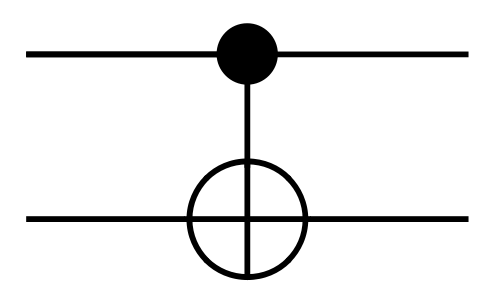
\includegraphics[width=0.2\textwidth]{cnot} 
    \end{center}
    You will have the chance to test it on this week's exercises.
\end{card}
\end{frame}


\subsection{More Gates} % swap, CCNOT, CSWAP, XX
\begin{frame}{More Gates}
\begin{cardTiny}
    As you dive deeper into the \qw, more gates will present themselves, you may even create your own (just remember their properties and do check if no one has come up with it yet).\\
    To spike your interest, here are a few more names you will eventually come across for quantum gates:
    \begin{itemize}
        \item SWAP
        \item Phase shift family
        \item CCNOT (AKA Toffoli)
        \item CSWAP (\textbf{C} usually stands for `Controlled')
        \item XX (not the band, no)
        \item Deutsch (not hardware implementation yet)
    \end{itemize}
\end{cardTiny}
\pagenumber
\end{frame}

\section{Exercises}
\begin{frame}{Exercises}
\begin{card}[Hands-on]
    This week you will start writing your first quantum gates, run simple circuits on a simulator, plot the readings. Do all of that in a real quantum device (and learn about real world concerns you should take).\\
    When you feel ready, move on to the \href{\weekThree/exercises/w3_01.ipynb}{exercises} and, if you feel stuck, you may look at the \href{\weekThree/exercises/w3_01_s.ipynb}{solutions}.
\end{card}
\pagenumber
\end{frame}

% \section{Universal \q Gates}
% \begin{frame}{FRAME}
% \begin{card}

% \end{card}
% \pagenumber
% \end{frame}




\section{Where to learn more?}
\begin{frame}{Where to learn more?}
\begin{card}
    \begin{itemize}
    \item \href{https://www.khanacademy.org/math/linear-algebra}{Khan Academy on Linear Algebra}
    \item \href{https://towardsdatascience.com/demystifying-quantum-gates-one-qubit-at-a-time-54404ed80640}{Medium article on common \q Gates}
    \item \href{https://www.quantiki.org/wiki/quantum-gates}{Quantiki entry on \q Gates}
    \end{itemize}
\end{card}
\end{frame}
\end{document}
